\documentclass[../index.tex]{subfiles}
 
\begin{document}


Мало кто знает, что история динамического языка началась задолго до появления автоматизированной системы <<Лицо Друга>>. Первые зачатки динамических форм родились в славном городе Ростов, более 10 лет назад.


Кирилл Борисович Кривошеев, создатель динамического языка,  в те времена работал начальником отдела внедрения и сопровождения автоматизированных систем Юго-Западного территориального банка ПАО Сбербанк. Работы было много и, не смотря на всю самоотверженность и трудолюбие сотрудников, на отдел постоянно поступали жалобы . И причина тому была воистину «сбербанковская»: с утра и до позднего вечера сотрудники разгребали сотни заявок от пользователей на просьбы разблокироваться в каких-либо системах. На одного сотрудника в день могло назначаться более 200 заявок. Звонили пользователи, просили разблокировать их учётные записи, по звонку регистрировались запросы, которые затем передавались в другие подразделения. Далее искали заявителя в базе и выясняли причину проблемы. А причины могли быть самые нелепые, например, пользователь вместо логина упорно вбивал какую-нибудь хрень.


Вся эта ситуация будоражила сознание Кирилла, а вокруг никто не желал пошевелить и пальцем, чтобы как-то улучшить процесс, зато ежедневных жалоб и нытья было вагон и маленькая тележка. 
И тут Кирилл начал задумываться о способах автоматизации процессов.

\section{Вижу цель не вижу препятствий}

В 2010 году Кирилл Борисович перешел на должность заместителя директора управления внедрения и сопровождения Юго-Западного территориального банка. После вступления в должность Кирилл стал отвечать за всю автоматизацию банка, и, помимо отдела внедрения и сопровождения, под его руководством оказалась диспетчерская служба.

Теперь он наблюдал за еще большим количеством сотрудников, страдающих от скучных рутинных процессов. 


Понимая, что если не он, то никто, Кирилл принялся за написание программы по оптимизации процесса разблокировки учетных записей. При этом стоит отметить, что на тот момент Кирилл Борисович толком не знал ни одного языка программирования, не считая языка PL+ , помеси SQL и объектно-ориентированного подхода, на котором были написаны многие автоматизированные системы. 


Писать на PL+ было не вариант, но Кирилла это не остановило. “Гугл в помощь” и вот наш герой уже шпарит свою первую программу на свежевученном языке программирования C\#. Всего было 25 программ для 25-ти автоматизированных систем. И эти 25 программ могли экономить для каждого пользователя примерно час жизни, которые ранее уходили на получение доступа, подачу заявки и ожидание в очереди на исполнение. Программа же справлялась с задачей всего за 30 секунд! 


“Зашибись!” — подумал Кирилл, и пошел продавать идею заместителю председателя банка. И тут барьеры на пути к цели вновь дали о себе знать. Задумка была отклонена, а вместо нее была дана рекомендация нанять побольше людей в контактные центры и научить их нормально работать… 


Вера в банковскую утопию, где сотрудники не должны были бы страдать от рутинных бессмысленных процессов, все же не покидала Кирилла. И он решил совершить ход конем. Удачным стечением обстоятельств явилось то, что в том году в банке по всей стране происходило довольно значимое событие: Программа глобального внедрения производственной системы в Сбербанке под руководством самого Германа Грефа. Данная система была вдохновлена лучшим практиками компании Тойота. Именно благодаря ей, и по сей день в банке проводится Гемба, - процесс, когда начальник сам становится за станок, чтобы понимать проблемы изнутри, испытывая их на личном опыте.


Вместе с Гембой пришло поручение сверху оптимизировать всё, что только можно оптимизировать, например, был процесс связанный с чековой книжкой: после каждой операции, в соответствии с нормативными документами нужно было распечатать чековую книжку, поставить печать, зарегистрировать ее и т.д. На*ера?! Клиент этого не хочет, потребности у него такой точно нет. А сотрудник тратил довольно много времени на эти бессмысленные процессы.  И вот, в рамках оптимизации, отменили сначала печати, а потом и вовсе чековые книжки.


Кириллу, как заместителю директора, также пришло поручение оптимизировать процессы внутри отделов. И тут, не растерявшись, Кирилл Борисович решил повторно презентовать свою идею, но только теперь уже напрямую в центральный аппарат. Идея была принята. Так появилась на свет программа B@nk Helper, программа, которая помогала пользователям быстро получить доступ в необходимую систему. 

\begin{figure}[h]
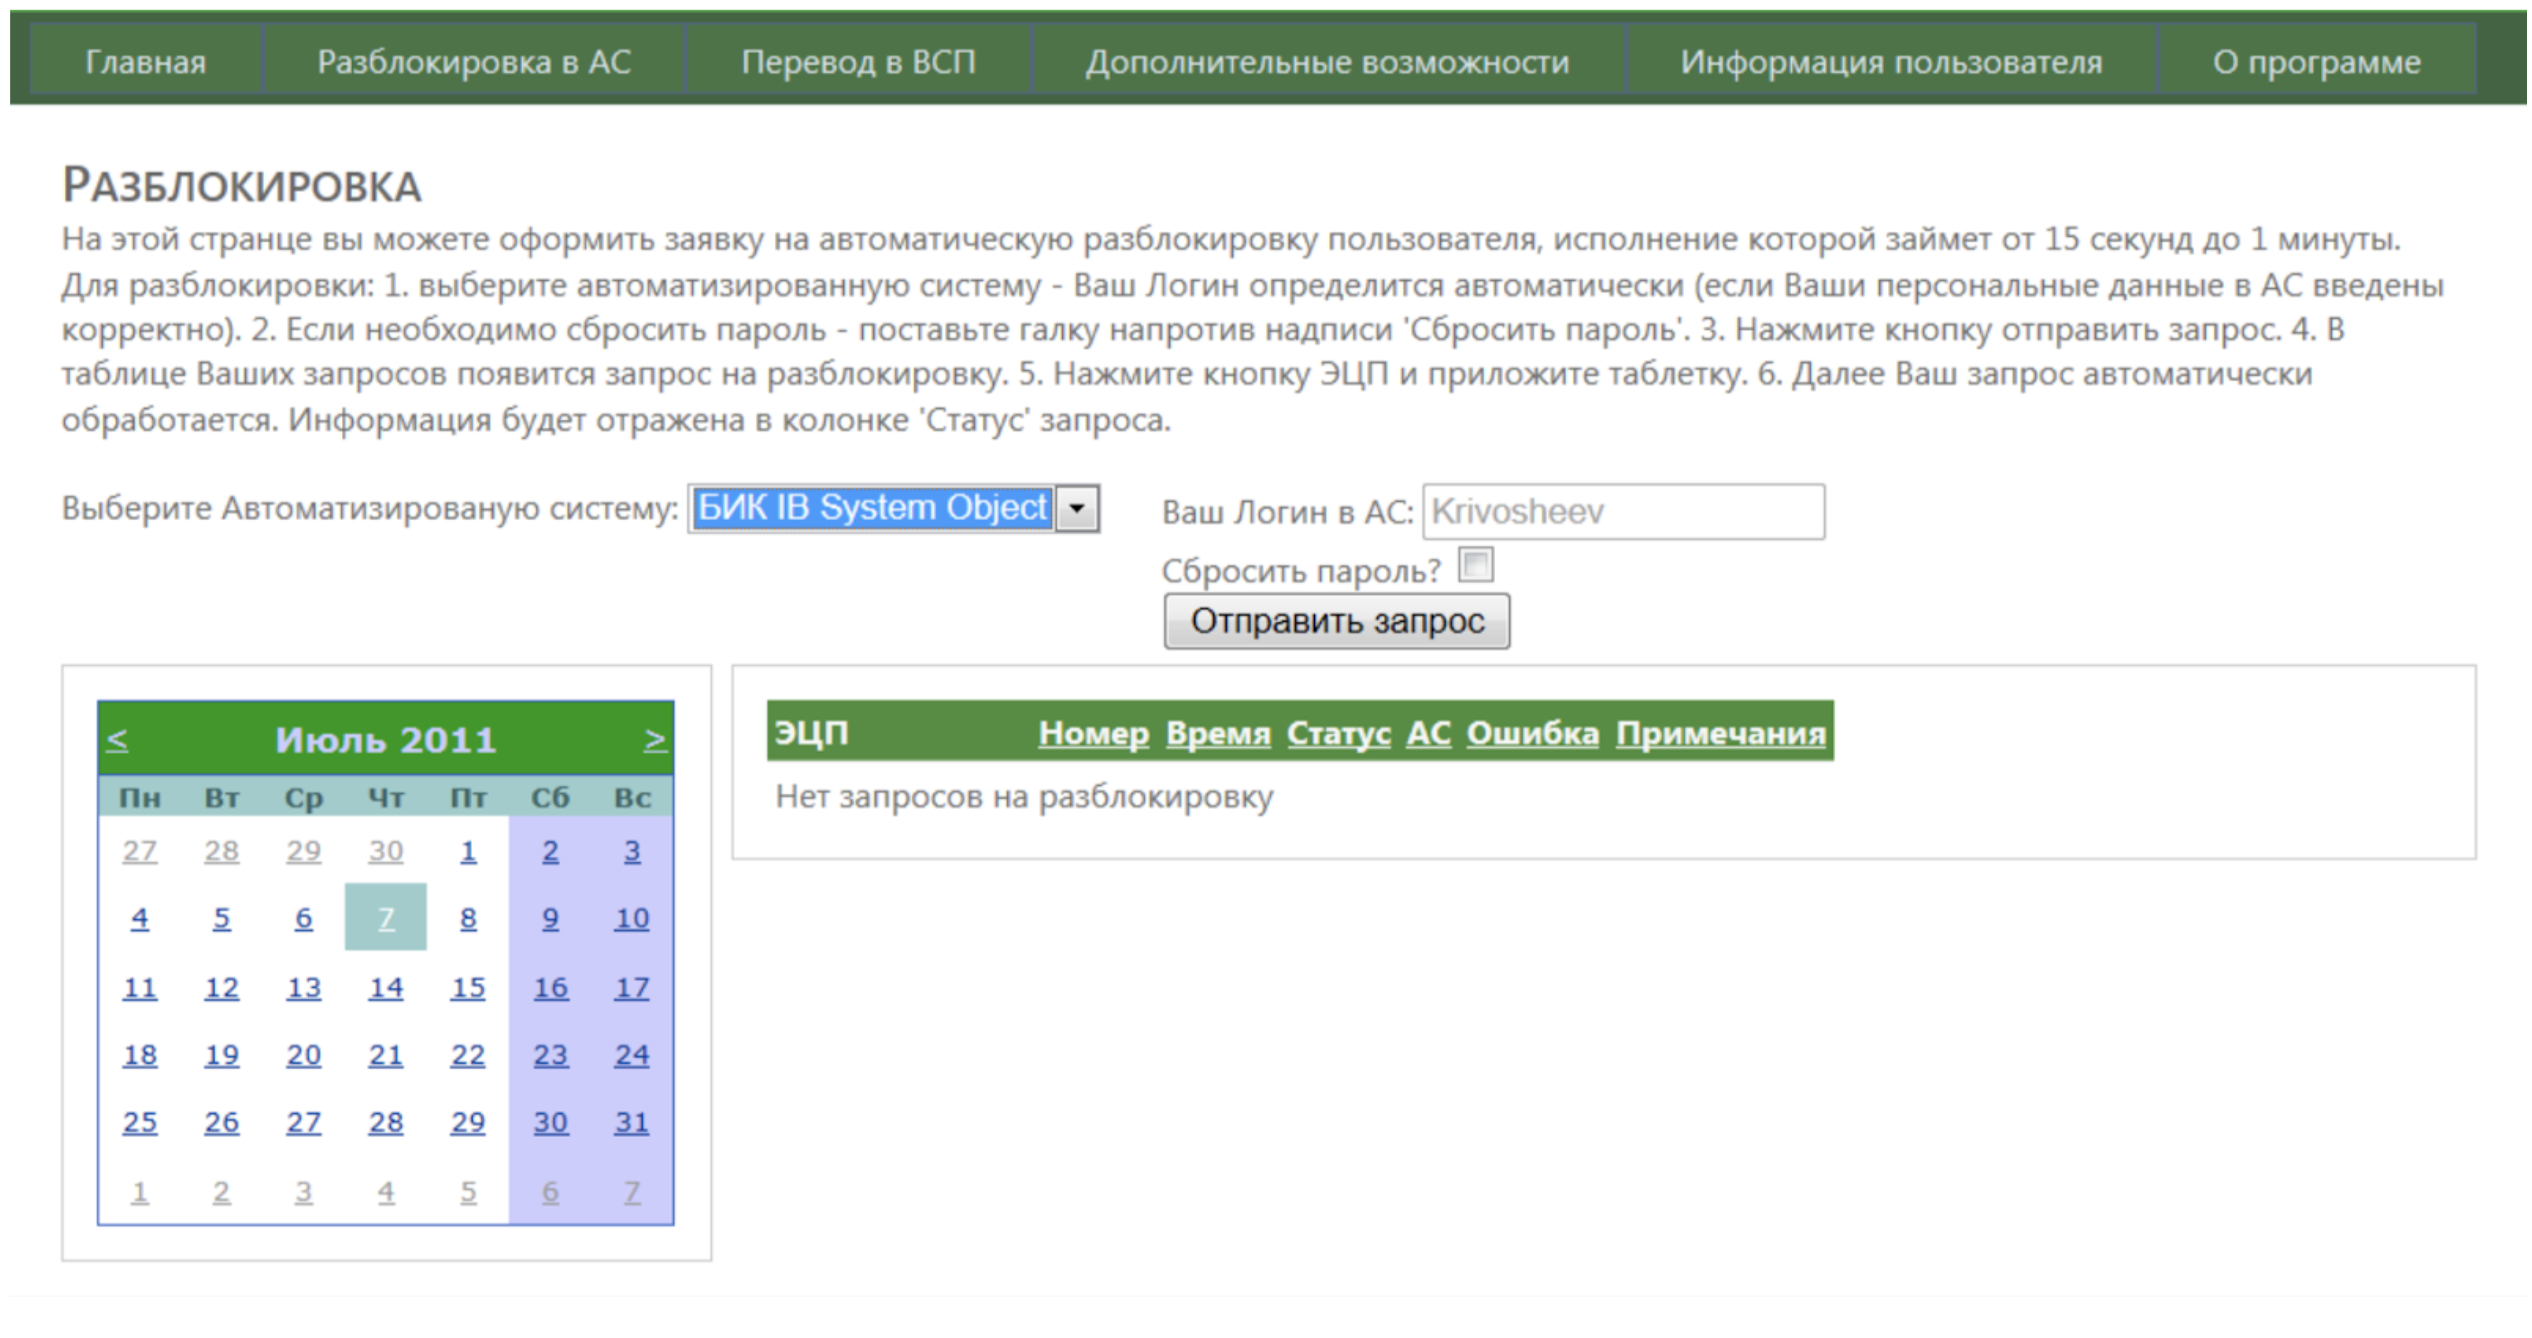
\includegraphics[width=0.9\textwidth]{bankhelper}
\centering
\end{figure}

\section{Первый успех и рождение динамических форм}

Итак, программа B@nk Helper была запущена и представлена всем заведующим филиалов банка в городе Ростов и, чтобы вы понимали, это 80 женщин (!). 
После презентации к Кириллу подошел директор, и сказал:
“Еще никогда в жизни я не видел такого количества одновременно оргазмирующих женщин!”.



И это было только начало. B@nk Helper сразу полюбился сотрудникам банка, но как говорится к хорошему привыкаешь быстро. Вскоре начали поступать запросы на дополнительные изменения в программе, например, добавить галочку или списочек. И Кирилл, конечно же,  совершенствовал B@nk Helper. Но изменения в системе давались не так просто, ведь приходилось вносить их в каждой форме для 25 однотипных автоматизированных систем. Так появился еще один процесс, который было необходимо оптимизировать. 



Кирилл Борисович начал думать над тем, как унифицировать процессы, как избавить себя от необходимости кодить каждый раз и не тратить на это уйму времени, а иметь возможность через простые настройки настраивать формы как надо. И именно такой способ настройки форм и придумал Кирилл. Способ, при котором не нужно было проводить ПСИ (приемо-сдаточные испытания), отдельно выводить функционал в промышленную эксплуатацию.  Формы программы можно было настроить в любой момент так, как необходимо. 



Запросы не прекращались, появилась потребность при изменении одного поля ввода, в зависимости от введённых в него данных автоматически подгружать другое поле ввода. Кирилл придумал как справиться и с этой задачей. Эти формы и стали первым прототипом динамических форм, таких, какими мы знаем их сейчас. 



Таким образом B@nk Helper стал прекрасным решением как для пользователей, так и для разработчиков. А Кирилл даже получил почетное звание “Инноватор Года”, которое записано в его паспорте участника  корпоративной системы работы с инновациями. Этот паспорт по сей день  бережно хранится шкафчике в кабинете Кирилла Борисовича. 

\begin{figure}[h]
	\includegraphics[width=0.9\textwidth]{bh_passport}
	\includegraphics[width=0.9\textwidth]{bh_passport_2}
	\centering
\end{figure}


В тоже время, помимо наград и всеобщего признания  Кириллу Борисовичу поступило официальное предложение о переезде в Москву для тиражирования  системы B@nk Helper во все территориальные банки.


\end{document}